\section{The Omega Equivalence Principle: From Great Circle to Spiral}

\begin{figure}[ht]
\centering
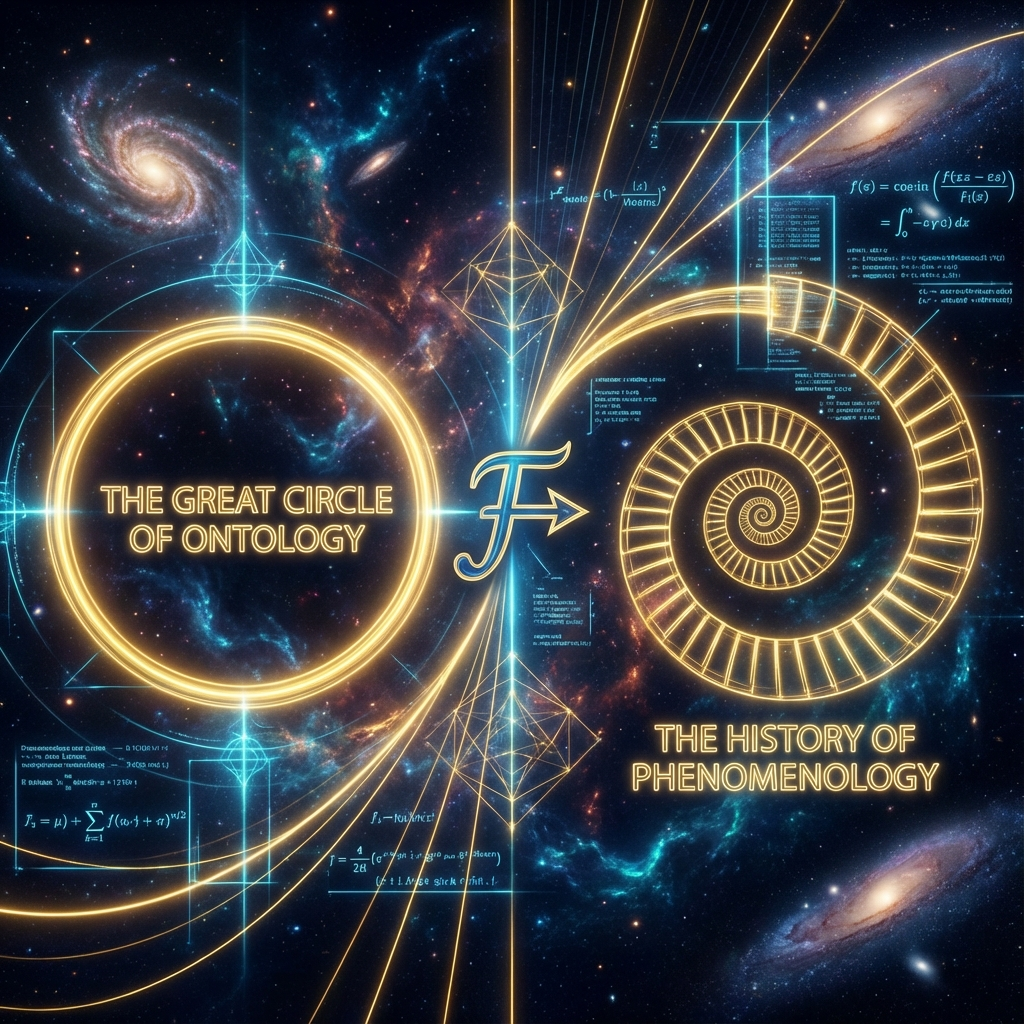
\includegraphics[width=0.8\textwidth]{assets/chapter05-05-omega-equivalence-principle.png}
\caption{Omega Equivalence Principle}
\end{figure}

In Section 5.4, we established the ``Total Budget Conservation'' axiom, pointing out that the universe's total energy (i.e., the total ontological information) is strictly constant ontologically, and the expansion and energy growth we observe arise from the relative contraction of measurement scales. However, this conservation law leaves a critical dynamical gap: How does a static, conserved ``1'' produce such a rich, dynamic evolutionary history with Fibonacci exponential growth in the phenomenal world?

This section will reveal the \textbf{core mathematical mechanism} of Omega Theory. We will prove that four seemingly distinct concepts in physics---state vectors in Hilbert space, geometry of high-dimensional spheres, spectral analysis (Fourier transform), and the Fibonacci spiral---are \textbf{Congruent} at the mathematical foundation. Cosmic evolution is essentially an \textbf{infinite non-ergodic Fourier analysis} performed on a \textbf{high-dimensional Great Circle}.

\begin{figure}[ht]
\centering
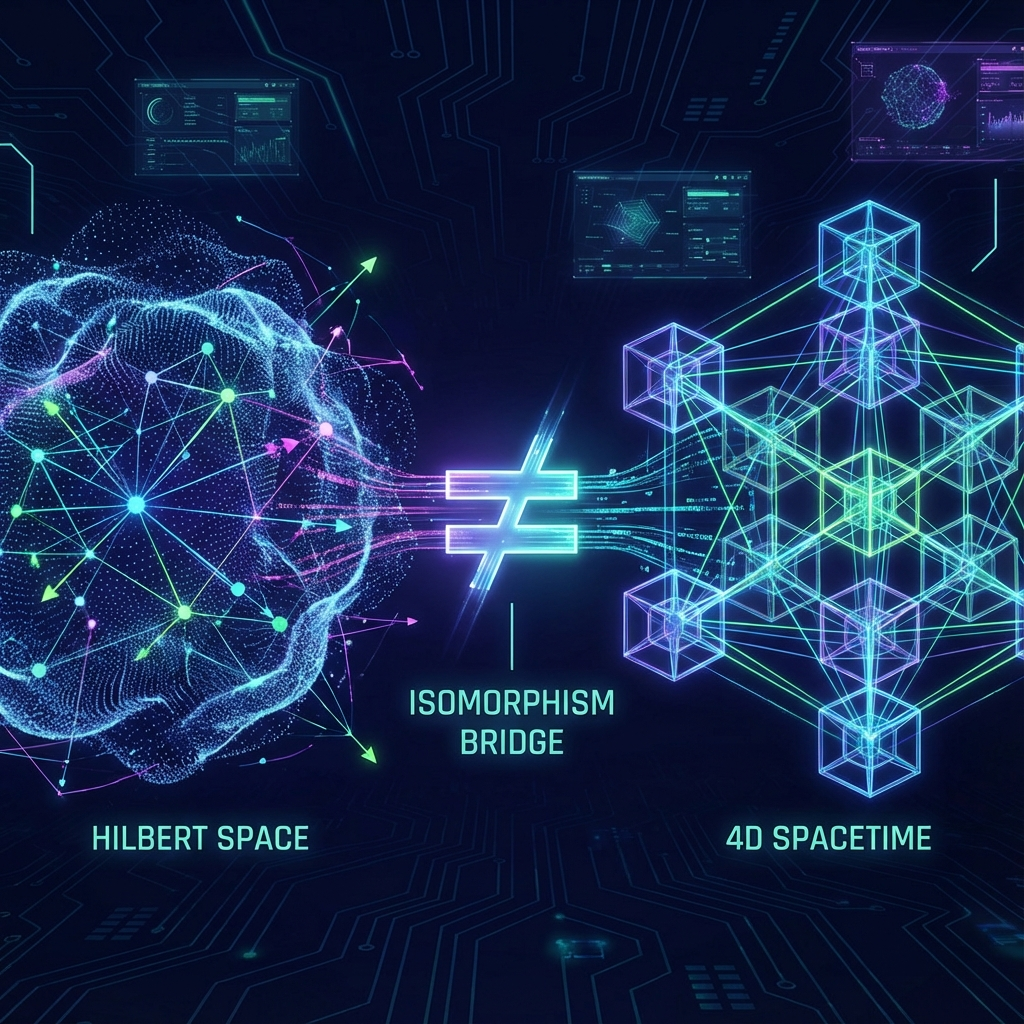
\includegraphics[width=0.8\textwidth]{assets/chapter05-05-hilbert-spacetime-bridge.png}
\caption{Hilbert Spacetime Bridge}
\end{figure}

\subsection{Isomorphism between Hilbert Space and High-Dimensional Spheres}

According to quantum mechanics axioms, the physical state of the universe is described by a single vector $|\Omega\rangle$ in Hilbert space $\mathcal{H}$. From the normalization condition $\langle \Omega | \Omega \rangle = 1$, we know that the endpoint of this vector is strictly constrained to the surface of a unit hypersphere $S^{\infty}$.

\[|\Omega\rangle \in \mathcal{H} \iff \text{Point on } S^{\infty}\]

This establishes \textbf{Geometric Rigidity}: the universe cannot ``grow'' or ``shrink'' ontologically; it can only ``rotate'' on the sphere. Any physical evolution operator $\hat{U}(\tau)$ is essentially an action of the special orthogonal group $SO(\infty)$ or unitary group $SU(\infty)$.
Therefore, \textbf{``Total Budget'' is the surface area of this hypersphere}. It neither produces nor annihilates; it is only redistributed.

\subsection{Time as Inverse Fourier Transform}

Then, if the ontology is a static sphere, where does ``time'' come from? What are ``events''?
In signal processing theory, any complex time-domain signal $f(t)$ can be decomposed into pure phase components $F(\omega)$ in the frequency domain through \textbf{Fourier transform}.
\[f(t) = \int F(\omega) e^{i\omega t} d\omega\]

In Omega Theory, we perform the inverse operation: \textbf{The universe's ontology is frequency-domain (static $|\Omega\rangle$), while the spacetime we perceive is time-domain (dynamic).}
When we say the universe is ``evolving,'' we are actually performing an \textbf{inverse Fourier transform} on the static vector $|\Omega\rangle$.

\begin{itemize}
\item \textbf{Static Spectrum}: Energy eigenstates $|E_n\rangle$ in Hilbert space and their weights $c_n$.
\item \textbf{Reading Process}: Unitary evolution operator $e^{-i E_n \tau}$ acts as scanning kernel.
\item \textbf{Dynamic History}: Output of Fourier transform, i.e., particle motion, wavefunction collapse, and historical events we see in spacetime.
\end{itemize}

\textbf{Conclusion}: Time is not a flowing entity; it is the \textbf{scanning pointer of spectral analysis}. Past, present, and future are merely interference patterns of the same set of spectra at different phase angles.

\subsection{Fibonacci Spiral: Non-ergodic Decomposition of the Great Circle}

Now, the crucial question arises: Why doesn't this scanning process repeat itself every period $T$ like ordinary circular motion (leading to Nietzschean ``eternal recurrence'')? Why does the universe exhibit irreversible innovation and growth?

The answer lies in the \textbf{number-theoretic properties of frequencies}.
If the Hamiltonian's energy spectrum $E_n$ consists of integers or rational numbers, the Fourier transform will trace a closed circle (or torus knot) in the complex plane. But in Omega Theory, according to the derivation in Chapter 1, the spectrum is generated by the \textbf{Golden Ratio $\phi$}:
\[E_n \propto \phi^n\]

When we perform Fourier superposition on a spectrum based on the irrational number $\phi$, the resulting trajectory no longer closes.
Consider the phase mapping on the complex plane:
\[z(\tau) = e^{i \cdot 2\pi \phi \cdot \tau}\]
As intrinsic time $\tau$ increases, this point is not drawing a circle but tracing a \textbf{Logarithmic Spiral} on a \textbf{Riemann surface}.

This is the geometric essence of \textbf{``Equivalence''}:
\textbf{Fibonacci Spiral $\equiv$ Infinite Non-ergodic Decomposition of the Great Circle}.

\begin{itemize}
\item \textbf{Great Circle}: Represents the sum of all possibilities in the universe (total budget $2\pi$).
\item \textbf{Decomposition}: Represents the observational slice at moment $\tau$. Each increase in $\tau$ corresponds to cutting an extremely thin slice from the great circle using the golden angle $\theta_g$.
\item \textbf{Infinite Non-ergodic}: Because $\phi$ is the ``most irrational'' number, these cut points never coincide; the spiral forever approaches the center (truth/Omega point) but never closes.
\end{itemize}

\subsection{Theorem 5.5: The Omega Equivalence Principle}

We summarize the above physical picture as Omega Theory's \textbf{Grand Equivalence Chain}. This is the ultimate formula connecting the algebraic foundations and dynamical evolution of this book.

\textbf{Theorem 5.5 (The Omega Equivalence Principle)}:
In an interactive computational universe, the following four mathematical structures are \textbf{Isomorphic} or \textbf{Dual} representations:
\[|\Omega\rangle_{\text{Vector}} \cong S^{\infty}_{\text{Sphere}} \cong \mathcal{F}_{\phi}[\text{Spectrum}] \cong \text{Spiral}_{\text{Evolution}}\]

\textbf{Physical Interpretation}:
\begin{enumerate}
\item \textbf{Ontology}: The universe is a static high-dimensional sphere (total budget conservation).
\item \textbf{Mechanism}: The universe expresses itself through $\phi$-based Fourier spectral analysis (great circle decomposition).
\item \textbf{Phenomenon}: In the observer's view, this manifests as Fibonacci spiral expansion in spacetime (light speed increase, universal growth, entropy-decreasing evolution).
\end{enumerate}

This principle completely eliminates the opposition between ``static universe'' and ``dynamic universe.'' \textbf{The universe is ontologically a static circle and epistemologically a dynamic spiral.} We feel we are experiencing time because we are being parsed bit by bit by this massive Fourier transform algorithm. We are travelers on that spiral infinitely approaching the center; each time we look back, we see a finer structure of the great circle.
